\section{Ziele}
\label{sec:Ziele}
\section{Theoretische Grundlagen}
\label{sec:Theorie}
Das Geiger-Müller-Zählrohr ist ein Messinstrument um die Intensität ionisierender Strahlung zu messen.
Bei einer Absorption eines $\alpha , \beta$ oder $\gamma$ Teilchens wird vom Zählrohr ein Impuls abgegeben und es lässt sich anhand der Impulse auf die Anzahl der Teilchen schließen.
\subsection{Aufbau und Funktionsweise}
\label{sec:Funktion}
Das Geiger Müller besteht aus einem Metallzylinder als Kathode (mit Radius $r_{\text{k}}$) und einem dünnen Metalldraht in der Mitte der als Anode (mit Radius $r_{\text{a}}$).
Innerhalb des Zylinders ist ein Gasgemisch aus einem Gas und einem Alkohol Anteil (siehe: \ref{sec:Nachentladung}) das von den eintreffenden Teilchen ionisiert werden kann.
Außen an die Anode und Kathode wird eine Spannung angelegt und ein Wiederstand geschaltet.
Durch die angelegte Spannung entsteht im Zählrohrvolumen ein Radialsymmetrisches E-Feld.
\begin{equation}
    E(r) = \frac{U}{r \ln\left(\frac{r_{\text{k}}}{r_{\text{a}}}\right)}
\end{equation}
\begin{figure}
    \centering
    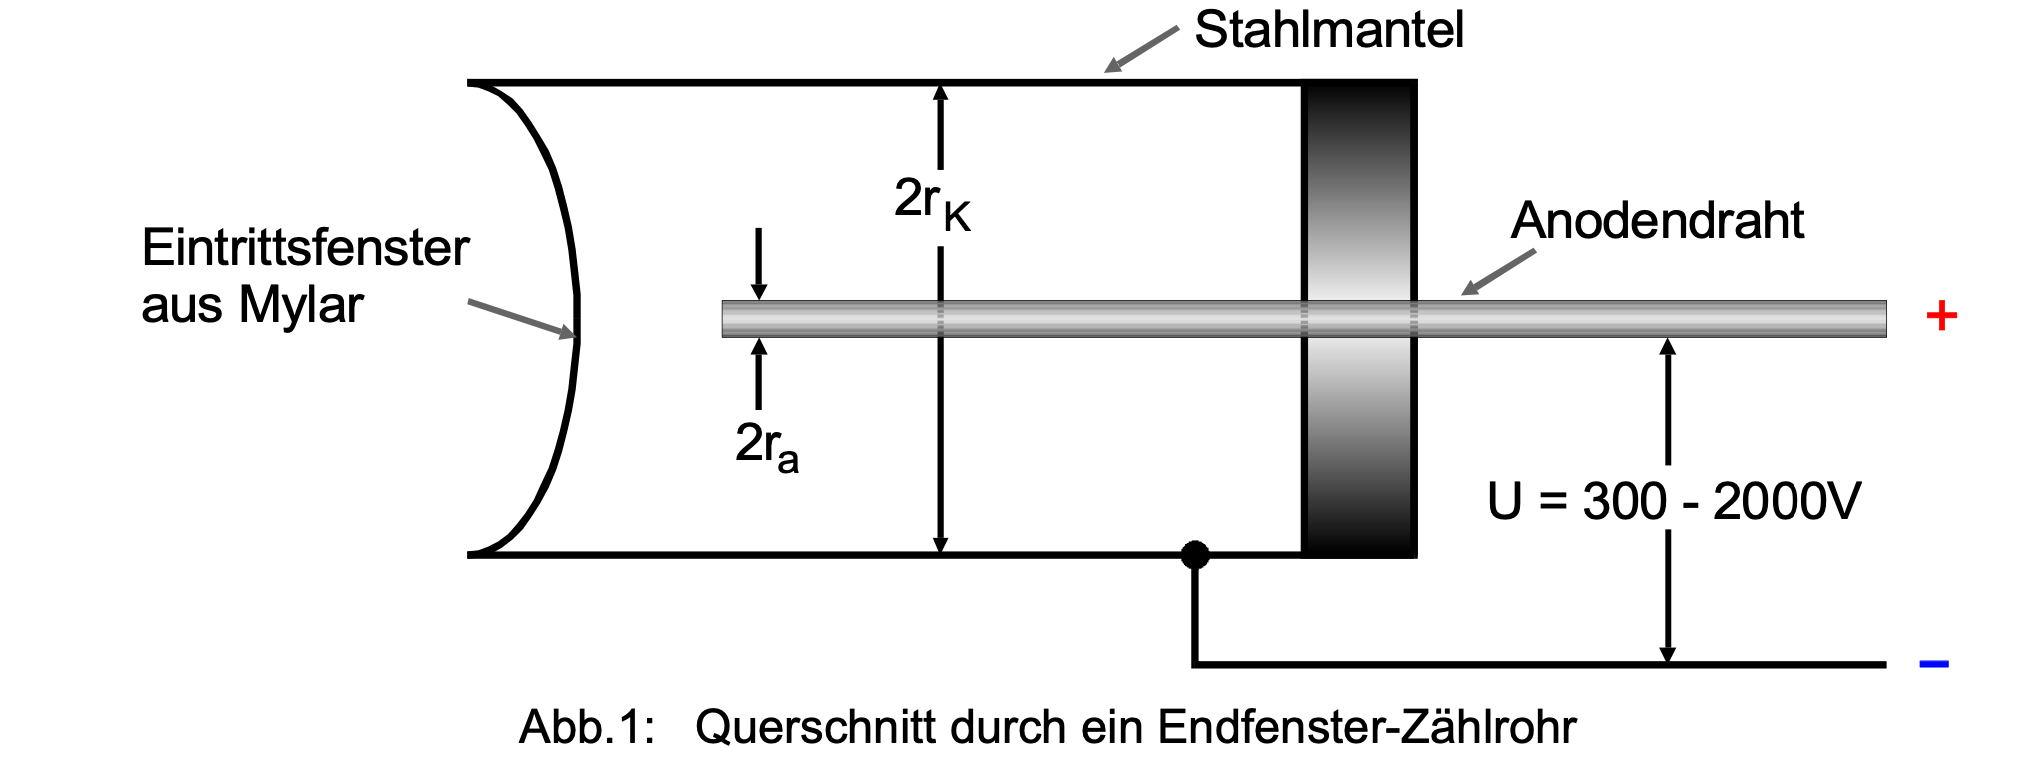
\includegraphics[width=0.3\textwidth]{bilder/Zaehlrohr_Querschnitt.png}
    \caption{Ein Zaehlrohr-Querschnitt. (Quelle \cite{Anleitung})}
    \label{fig:Zaehlrohr}
\end{figure}
Die Messung der einfallenden Teilchen und somit der Intensität ist stark abhängig von der angelegten Spannung.
\begin{figure}
    \centering
    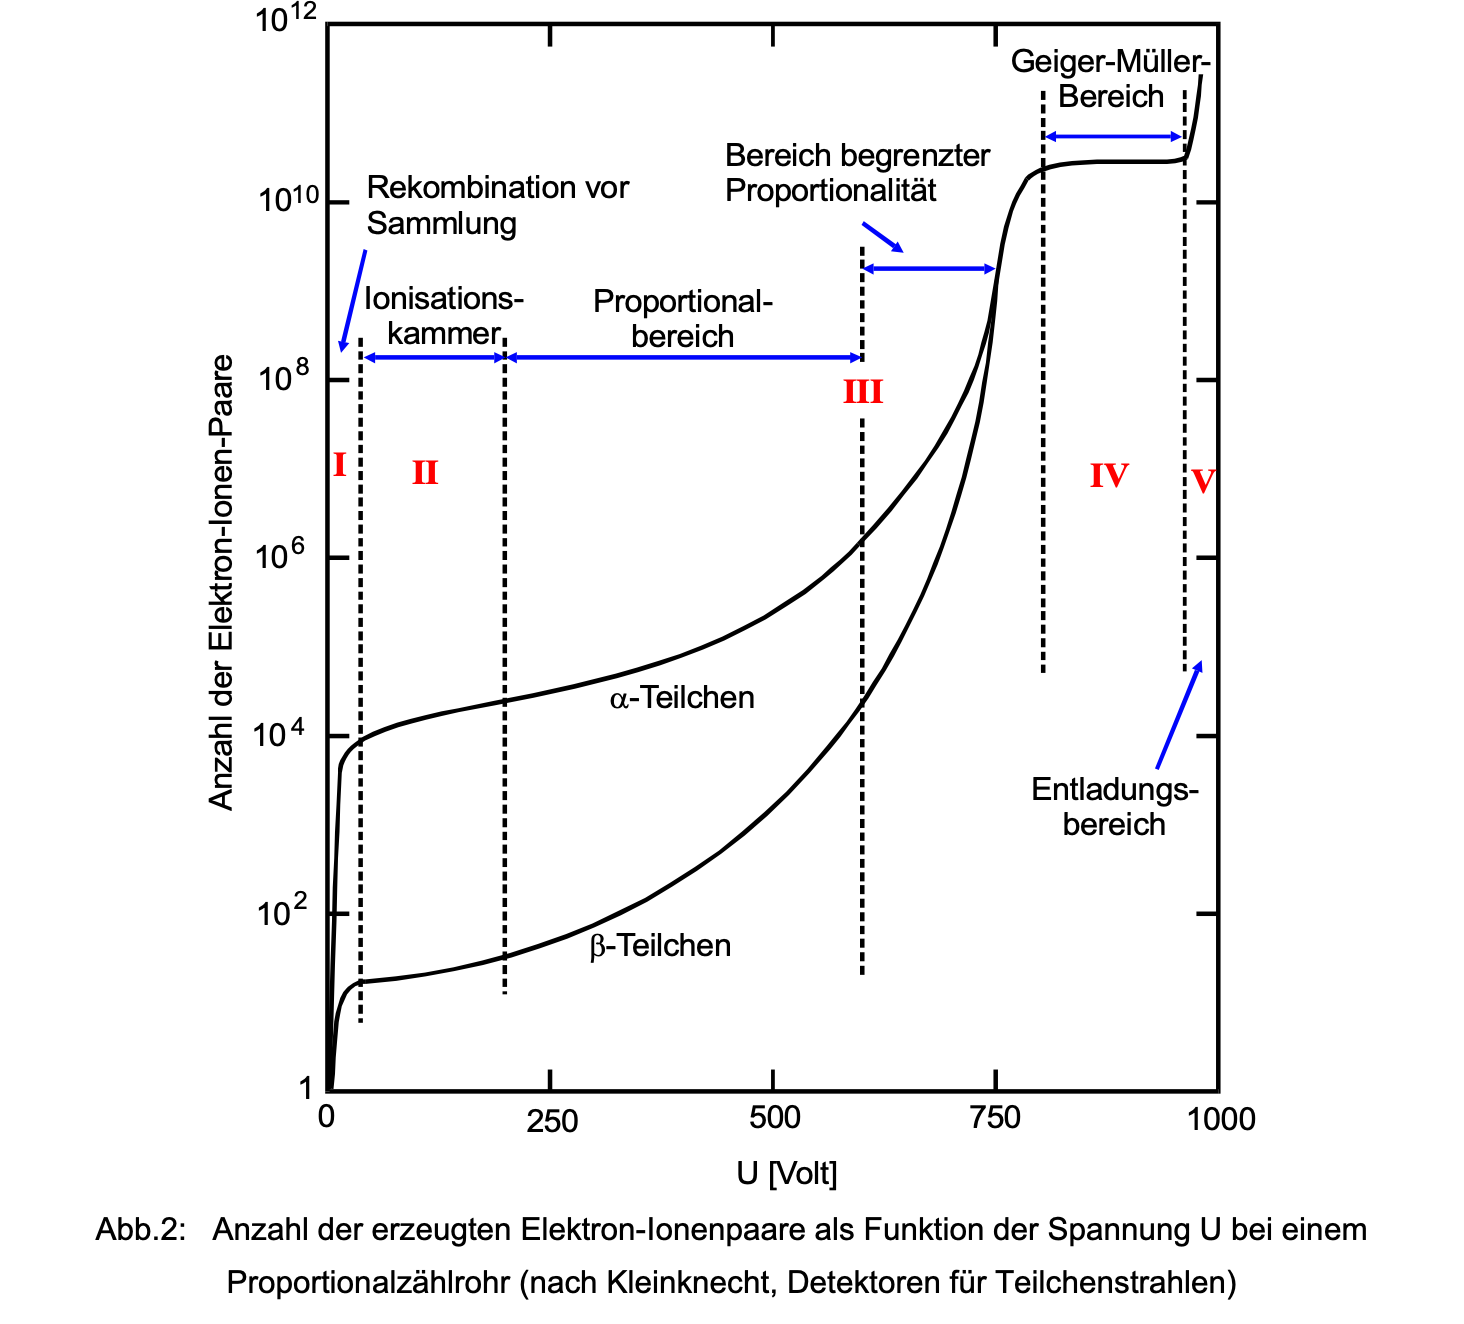
\includegraphics[width=0.5\textwidth]{bilder/Anzahl_der_Elektronen.png}
    \caption{ Anzahl der Elektronen-Ion-Paare. (Quelle \cite{Anleitung})}
    \label{fig:Anzahl_der_Elektronen}
\end{figure}
Wenn zu Beginn nur eine Sehr schwache Spannung angelegt ist reicht diese nicht aus um die Elektron Ion Paare zu trennen und sie Rekombinieren direkt wieder (Bereich I).
In diesem Bereich steigt die Anzahl der detektierten Elektronen schnell an, da mit der steigenden Spannung die Wahrscheinlichkeit des Rekombinierens schnell sinkt.
In dem Bereich (II) unmittelbar nachdem die Rekombinationswahrscheinlchikeit gegen Null gelaufen ist, können mit dem Zählrohr nur sehr hohe Strahlungsintensitäten gemseen werden und Zählrohre dieser Art werden Ionisationskammer genannt.
Wenn die Spannung weiter erhöht wird nehmen die Elektronen aus den Ionisationen zwischen zwei Atomen genug Energie auf um das nächste Atom das sie stoßen zu ionisieren.
Durch diese sogenannte Stoßionisation entsteht ein lawinenartiger Anstieg der Anzahl der Elektronen, dieses Phänomen wird die Townsend-Lawine genannt.
Auch wenn in diesem Intervall pro Teilchen sehr viele Elektronen entstehen ist der gemessene Ladungsimpuls immer noch proportional zur Energie des einfallenden Teilchens.
Daher lässt sich in diesem Bereich sowohl die Intensität als auch die Teilchenenergie messen und Zählrohre die in diesem Bereich arbeiten werden Proportionalitätszählrohr genannt.
Wenn die Spannung den Proportionalitätsbereich übersteigt wird der Ladungsimpuls unabhängig von der Energie des einfallenden Teilchens und der Auslösebereich beginnt.
Der Auslösebereich ist der Arbeitsbereich des zu untersuchenden Geiger-Müller-Zählrohres.
In diesem Bereich werden die Atome im Gas nicht nur durch Elektronen ionisiert, sondern für die Stoßionisation nehmen die Elektronen so viel Energie auf, dass bei der Ionisation auch UV-Photonen frei werden.
Die entstandenen UV-Photonen  können sich im Zählrohr unabhängig von dem E-Feld bewegen und weitere Teilchen ionisieren, daher wird in diesem Bereich das gesamte Zählrohr Volumen ionisiert.
Nun ist der zu messende Ladungsimpuls nich abhängig von der Teilchenenergie aber abhängig vom Volumen des Zählrohrs, daher lässt sich mit dem Geiger-Müller-Zählrohr nur die Strhlungsintensität messen.
Wenn die Spannung über diesen Bereich erhöht wird kann das Zählrohr nicht mehr richtig arbeiten und durch eine kontinuierliche Ionisation im Zählrohrvolumen wird jenes zerstört.
\subsubsection{Totzeit}
Wenn die Atome im Zählrohr ionisiert werden, können die beweglichen Elektronen schnell zum Anodendraht in der Mitte der Zählrohrs gehen, aber die Ionen bleiben wegen ihrer größeren Masse noch länger im Zählrohrvolumen.
Durch den sich aus den Ionen bildenden Schlauch von positiven Ladungen um den Anodendraht wird das E-Feld im inneren geschwächt und es kann keine Stoßionisation stattfinden.
Daher kann für ein Zeitintervall $T_{\text{tot}}$ kein einfallendes Teilchen detektiert werden.
Erst wenn die Ionen im Zählrohr wieder vollstaändig neutralisiert sind kann der Ladungsimpuls wieder seine ursprüngliche Höhe erreichen.
Dadurch eintsteht zwischen den Pulsen auch eine sogenannte Erholungszeit $T_{\text{E}}$ in der nur geschwächte Ladungsimpulse stattfinden.
\begin{figure}
    \centering
    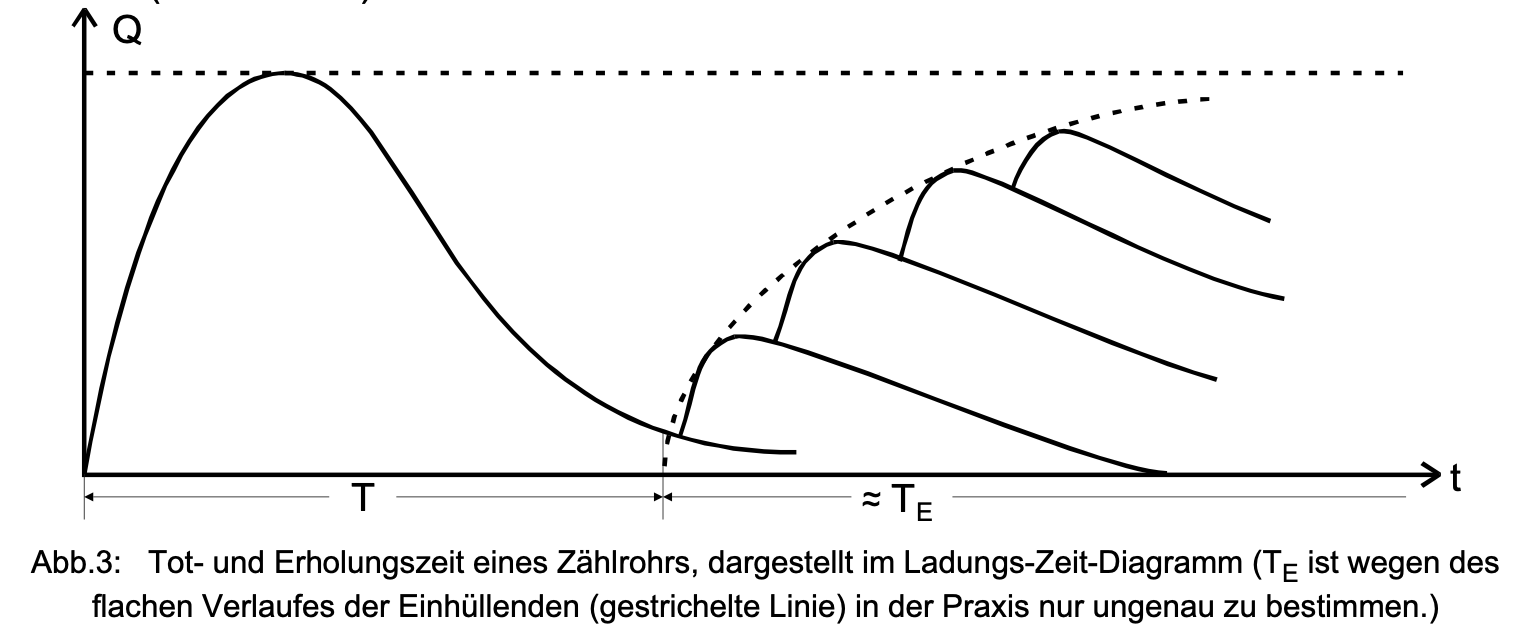
\includegraphics[width=0.5\textwidth]{bilder/Totzeit_Erholungszeit.png}
    \caption{Ein Graph. (Quelle \cite{Anleitung})}
    \label{fig:Totzeit_Erholungszeit}
\end{figure}
\subsubsection{Nachentladung}
\label{sec:Nachentladung}
Bei der Neutralisation der Ionen an der Metallkathode, kann es vorkommen, dass durch überschüssige Energie Elektronen aus dem Metall augelöst werden.
Die ausgelösten Elektronen müssen dann das gesamte Zählrohr durchhlaufen um zum Anodendraht zu gelangen und ionisieren auf ihrem Weg neue Atome.
Dadurch entstehen nach der ursprünglichen Ladungslawine noch weitere Ladungslawinen und man detektiert die sogenannten Nachentladungen.
Da die Ladungsimpulse nicht zu unterscheiden sind von den Ladungsimpulsen durch die einfallenden Ionisierenden Teilchen, verfälschen die Nachentladungen die Messung.
Um Nachentladungen zu verhindern wird dem Gas noch ein Alkoholanteil hinzugemischt.
Wenn nun die Ionen auf dem Weg zum Metallmantel mit einem Alkoholmolekül zusammenstoßen ionisieren sie ein Atom des Alkohols und neutralisieren sich dabei.
Der Ionisierte Alkohol wandert nun zum Kathodenmetall und wird dort neutralisiert, wobei kein Elektron aus dem Metall ausgelöst wird, sondern lediglich der vielatomige Alkohol zu Schwingungen angeregt wird.
\subsection{Charakteristik Geiger-Müller-Zählrohr}
\begin{figure}
    \centering
    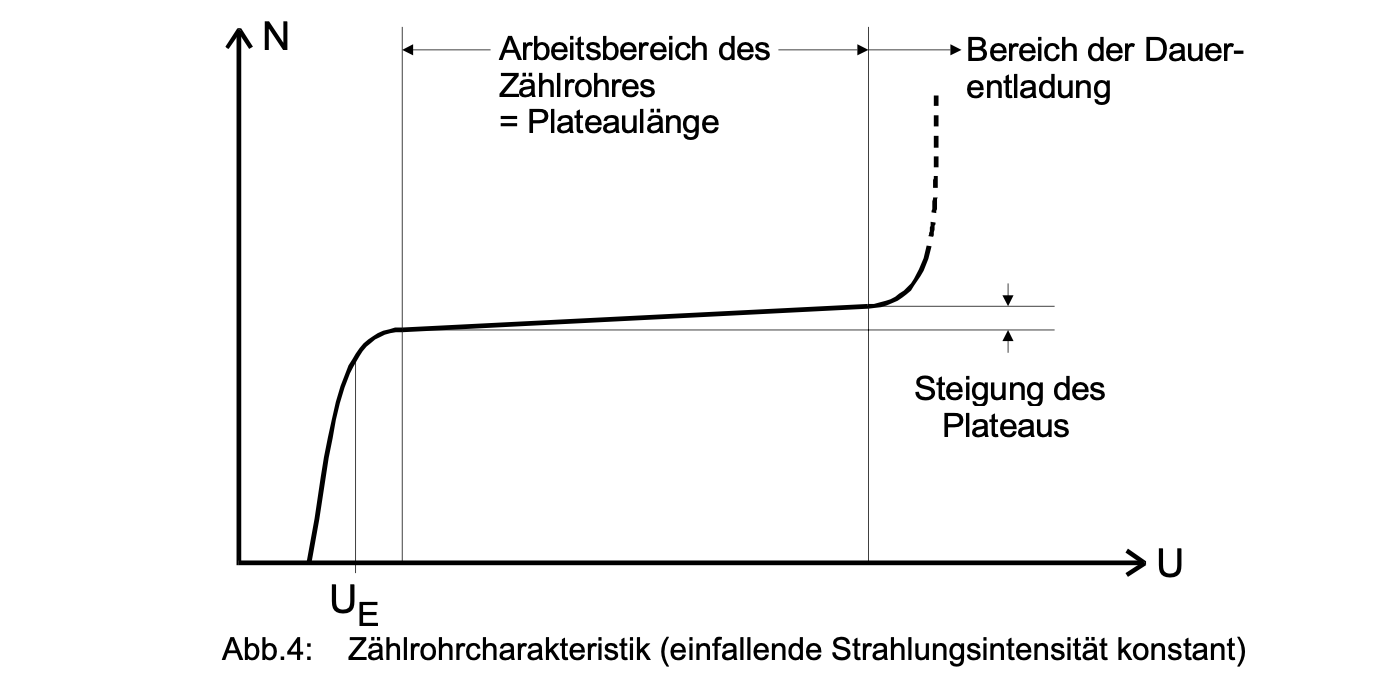
\includegraphics[width=0.5\textwidth]{bilder/Zaehlrohr_N_U_Graph.png}
    \caption{Ein N-U-Graph. (Quelle \cite{Anleitung})}
    \label{fig:Zaehlrohr_N_U_Graph}
\end{figure}
Wenn die Spannung wie in Kapitel \ref{sec:Funktion} beschrieben den Auslösebereich erreicht beginnt auch der Arbeitsbereich des Geiger-Müller-Zählrohres (Abb. \ref{fig:Zaehlrohr_N_U_Graph}).
Wenn ein Zählrohr optimal arbeitet, sollte der lineare Bereich im Arbeitsberieich des Geiger-Müller-Zählrohrs eine Steigung von Null haben.
Dieser lineare Bereich, der Plateau genannt wird, hat aber in der Realität immer eine kleine Steigung die auf Effekte wie die Nachentlacdung zuruückzuführen ist.
\subsection{Ansprechvermögen}
Das Ansprechvermögen eines Geiger-Müller-Zählrohrs hängt mit der Wahrscheinlichkeit verschiedene  Teilche  zu detektieren zusammen.
Für alpha und beta Teilchen ist das Ansprechvermögen im GM-Zählrohr annähernd 100\%, da wenn ein Teilchen dieser Art in das Zählrohr eindringt es fast immer detektiert wird.
Um dafür zu sorgen dass die Teilchen in das Zählrohr eindringen können und das Elektrische Feld im innern weiterhin bestehen bleibt, wird eine dünne Mylar Folie genutzt.
Die Mylar Folie sorgt dafür dass auf der Seite der Probe die Teilchen in das Zählrohrvolumen dringen können aber kein Gas austritt und der Strom weiterhin fließen kann.
Für Gamma Strahlung die in das Zählrohr eindringt ist das Ansprechvermögen ungefähr 1\%, da die Wahrscheinlichkeit dass Photonen ein Gas ionisieren sehr gering ist.